\section{Oscillatore armonico 1D}
Così come nell'oscillatore armonico classico, l'energia del sistema è data da energia cinetica più un'energia potenziale proporzionale al quadrato dello spostamento:
\[
    \H = \frac{\hat p^2}{2m} + \half m \omega^2 \hat x^2
\]
Risulta comodo introdurre gli operatori di creazione e di distruzione:
\begin{align}
    \hat a^\dag &= \sqrt{\frac{m \omega}{2 \hbar}} \left( \hat x - \frac{i}{m \omega} \hat p \right) \\
    \hat a &= \sqrt{\frac{m \omega}{2 \hbar}} \left( \hat x + \frac{i}{m \omega} \hat p \right)
\end{align}
Questa è una trasformazione canonica da $(\hat x, \hat p)$ a $(\hat a^\dag, \hat a)$ invertibile come segue:
\begin{align}
    \hat x &= \sqrt{\frac{\h}{2m\omega}}(\hat a^\dag + \hat a) \\
    \hat p &= i\sqrt{\frac{\h m\omega}{2}}(\hat a^\dag - \hat a)
\end{align}
Si può verificare che:
\[
    \left[ \hat a, \hat a^\dag \right] = 1
\]
Per un sistema con autostati discreti risulta che questi operatori incrementano o decrementano l'autovalore dell'energia di un autostato $|n\ket$:
\begin{align*}
    \hat a |n\ket &= \sqrt{n} |n-1\ket \\
    \hat a^\dag |n\ket &= \sqrt{n+1} |n+1\ket
\end{align*}
Infine, posto $\N = \hat a^\dag \hat a: \N\state n = n\state n$, risulta:
\[
    \H = \h\omega \l \hat N + \half\Id \r
\]

\subsection*{Zero point energy}
L'energia dell'oscillatore armonico quantistico non può essere nulla, altrimenti si vuolerrebbe il principio d'indeterminazione. Infatti l'energia minima è:
\(
    E_0 = \frac{1}{2} \hbar \omega
\)
E i valori dell'energia sono quantizzati e sempre multipli di questo $E_0$. \\
Questi valori di energia sono autovalori di autostati nella base delle energie, generata dall'hamiltoniano. \\
Risultano questi fatti:
\begin{align*}
    \hat a |0\ket = 0 \\
    \hat a^\dag |0\ket = |1\ket \\
    \hat a^\dag |1\ket = \sqrt{2} |2\ket \\
    |n\ket = \frac{(\hat a^\dag)^n}{\sqrt{n!}} |0\ket \\
\end{align*}
Altre coses:
\[
    \bra x | \hat a | 0 \ket = 0 \implies x \bra x | 0 \ket + \frac{i}{m\omega} \bra x | \hat p | 0 \ket = 0
\]
Sia $\vphi_0(x) = \bra x | 0 \ket$, allora:
\[
    x \vphi_0(x) + \frac{\hbar}{m \omega} \deriv[x]{} \vphi_0(x) = 0
\]
Siccome $\frac{\hbar}{m \omega}$ è una lunghezza al quadrato, si chiama $\xi = \sqrt{\frac{\hbar}{m \omega}}$ la lunghezza caratteristica e si risolve l'equazione differenziale (esercizio). Risulta:
\[
    \vphi_0(x) = A e^{-\frac{x^2}{2 \xi^2}}
\]
con $A = \frac{1}{(\pi \xi^2)^{1/4}}$ per la normalizzazione. \\
Quello trovato è lo stato fondamentale dell'oscillatore armonico quantistico in rappresentazione di posizione.

\begin{tikzpicture}[scale=1]
    % axes
    \draw[->] (-3.2,0) -- (3.2,0) node[right] {$x$};
    \draw[->] (0,-1.2) -- (0,5.2) node[above] {$y$};
    % ticks
    \foreach \x in {-3,-2,-1,1,2,3}
        \draw (\x,0.08) -- (\x,-0.08) node[below,font=\small] {};
    \foreach \y in {0,1,2,3,4,5}
        \draw (0.08,\y) -- (-0.08,\y) node[left,font=\small] {};
    % curves
    \draw[domain=-2.2:2.2,smooth,variable=\x,blue,thick] plot (\x,{(\x)*(\x)});
    \node[anchor=west,blue,font=\small] at (2.3,{2.3*2.3}) {$y=x^2$};
    \draw[domain=-2.5:2.5,smooth,variable=\x,red,thick]  plot (\x,{exp(-(\x)*(\x))+1});
    \node[anchor=west,red,font=\small] at (2.5,{exp(-2.3*2.3)+1.3}) {$y=e^{-x^2}+1$};
    % horizontal asymptote for the gaussian
    \draw[dashed,gray] (-3.2,1) -- (3.2,1) node[anchor=west,gray,font=\small] {};
    \draw (1,1) -- (1,0) node[left,font=\small] {};
    \draw (-1,1) -- (-1,0) node[left,font=\small] {};
\end{tikzpicture}

Quel che risulta per lo stato 0 è che siccome una particella quantistica è delocalizzata, essa ha un comportamento simile a una particella classica con abbastanza energia da potersi muovere nella zona di delocalizzazione, ovvero una particella che ha energia $E_0$.
Alcuni risultati utili:
\[
    \vphi_1(x) = \bra x | 1 \ket = \frac{\sqrt{2} x}{\xi}\vphi_0(x)\ \ \ \text{fare tutti i conti intermedi please}
\]
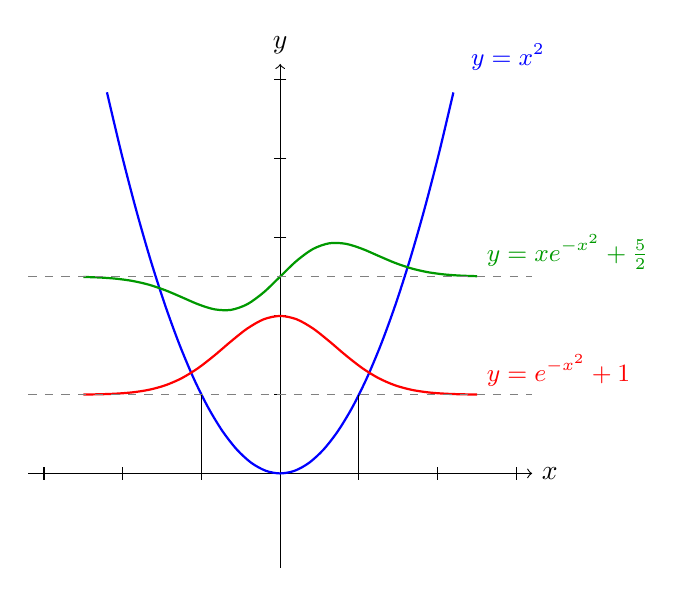
\begin{tikzpicture}[scale=1]
    % axes
    \draw[->] (-3.2,0) -- (3.2,0) node[right] {$x$};
    \draw[->] (0,-1.2) -- (0,5.2) node[above] {$y$};
    % ticks
    \foreach \x in {-3,-2,-1,1,2,3}
        \draw (\x,0.08) -- (\x,-0.08) node[below,font=\small] {};
    \foreach \y in {0,1,2,3,4,5}
        \draw (0.08,\y) -- (-0.08,\y) node[left,font=\small] {};
    % curves
    \draw[domain=-2.2:2.2,smooth,variable=\x,blue,thick] plot (\x,{(\x)*(\x)});
    \node[anchor=west,blue,font=\small] at (2.3,{2.3*2.3}) {$y=x^2$};
    \draw[domain=-2.5:2.5,smooth,variable=\x,red,thick]  plot (\x,{exp(-(\x)*(\x))+1});
    \node[anchor=west,red,font=\small] at (2.5,{exp(-2.3*2.3)+1.3}) {$y=e^{-x^2}+1$};
    \draw[domain=-2.5:2.5,smooth,variable=\x,green!60!black,thick] plot (\x,{(\x)*exp(-(\x)*(\x))+2.5});
    \node[anchor=west,green!60!black,font=\small] at (2.5,{2.3*exp(-2.3*2.3)+2.8}) {$y=x e^{-x^2}+\frac{5}{2}$};
    % horizontal asymptote for the gaussian
    \draw[dashed,gray] (-3.2,1) -- (3.2,1) node[anchor=west,gray,font=\small] {};
    \draw[dashed,gray] (-3.2,2.5) -- (3.2,2.5) node[anchor=west,gray,font=\small] {};
    \draw (1,1) -- (1,0) node[left,font=\small] {};
    \draw (-1,1) -- (-1,0) node[left,font=\small] {};
\end{tikzpicture}


Si può ricavare anche una formula generale:
\[
    \vphi_n(x) = \bra x | n \ket = \frac{1}{\pi^{1/4}\sqrt{2^n n!}} \frac{1}{\xi^{n+1/2}}(x-\xi^2 \deriv[x]{} )^n e^{-\frac{x^2}{2 \xi^2}}
\]
che, all'atto pratico, è una successione di funzioni oscillanti con frequenza sempre più alta.

Risulta inoltre che, $\bra n | \hat x | n \ket = 0$ e $\bra n | \hat p | n \ket = 0$.

\subsection*{Dinamica}
Risulta, passando dalla rappresentazione di Schrödinger a quella di Heisenberg:
\[
    i\hslash \tderiv{} \hat a_H = \U^\dag[\hat a, \hat H]\U = \U^\dag[\hat a, \hslash \omega(\hat a^\dag \hat a + \half)]\U = \hslash \omega \U^\dag \hat a \U = \hslash \omega \hat a_H
\]

E quindi
\[
\begin{cases}
        \hat a_H = \hat a e^{-i\omega t}\\
        \hat a_H^\dag = \hat a e^{i\omega t}
\end{cases}
\]
\[
    \hat X = \sqrt{\frac{\hslash}{2m\omega}}(\hat a + \hat a ^\dag) \implies \hat X_H = \sqrt{\frac{\hslash}{2m\omega}}(\hat a e^{-i\omega t} + \hat a ^\dag  e^{i\omega t})
\]
Al ché
\[
\begin{cases}
    \hat a = \frac{1}{\sqrt{2m\hslash\omega}}(m\omega \hat X + i \hat P)\\
    \hat a^\dag = \frac{1}{\sqrt{2m\hslash\omega}}(m\omega \hat X - i \hat P)
\end{cases}
\ \implies \ 
\begin{cases}
    \hat X_H(t) = \hat X \cos (\omega t) + \frac{\hat P}{m\omega}\sin (\omega t)\\
    \hat P_H(t) = 
\end{cases}
\]

\subsubsection*{Un Esempio, e i polinomi di Hermite}
\textit{Sia $|\psi(0)\ket = \frac{1}{\sqrt 2}(|0\ket + |1\ket)$. Allora}
\[
    |\psi (t) \ket = \U(t) |\psi(0)\ket = \sqrthalf e^{-i\omega t (\N + \sqrthalf)} = \sqrthalf\left(e^{-i\omega t/2}\state 0 + e^{-3i\omega t/2}\state 1\right)
\]
allora
\[
    \bra \hat X \ket = \bra \psi(t) | \hat X | \psi (t) \ket = \]\[
    \sqrt{\frac{\hslash}{8m\omega}}\left(e^{i\omega t/2}\dstate 0 + e^{3i\omega t/2}\dstate 1\right)(\hat a + \hat a^\dag) \left(e^{-i\omega t/2}\state 0 + e^{-3i\omega t/2}\state 1\right) = \]\[
    \sqrt{\frac{\hslash}{8m\omega}}(e^{-i\omega t} + e^{i\omega t}) = \sqrt{\frac{\hslash}{2m\omega}} \cos(\omega t)
\]
Che coincide con l'oscillatore classico!\\
Passiamo a questo:
\[
    \H\vphi = E\vphi \]\[
    -\frac{\hslash^2}{2m} \sderiv[x] \vphi + \half m\omega^2 x^2 \vphi = E\vphi
\]
Si può ricondurre a 
\[
    u'' + (\varepsilon - \xi^2)u = 0
\]
e ponendo $u(\xi) = H(\xi)e^{-\xi^2/2}$:
\[
    H'' - 2\xi H' + (\varepsilon - 1)H = 0
\]
risulta che, se $\varepsilon = 2n + 1$:
\[
    H_n(\xi) = (-1)^n e^{-\xi^2}\frac{d^n}{\xi^n}e^{-\xi^2}
\]
sono soluzione, e sono chiamati polinomi di Hermite. Si ha
\[
    \sum_{n=0}^{\infty}\frac{H_n(\xi) u^n}{n!}=e^{-u^2+2u\xi}
\]
ma che cacco

I polinomi di Hermite si possono calcolare in modo ricorsivo:
\[
    H_n' = 2nH_{n-1}\]\[
    H_{n+1}(\xi) = 2\xi H_n(\xi) - 2nH_{n-1}(\xi)
\]
con $H_0 = 1$ e $H_1 = 2\xi$.